\chapter{Resultados y Análisis}
\label{cap:resultados}

En este capítulo se presentan y analizan los resultados obtenidos con el simulador BCH desarrollado. Se examina el rendimiento del código en la corrección de errores (BER y CWER) y se evalúa la eficiencia computacional, siguiendo dos enfoques complementarios.

\section{Metodología Experimental}

Para evaluar el rendimiento, se ha implementado un entorno de simulación basado en el método de Montecarlo, el cual sigue un flujo de: generación de información, codificación, simulación del canal ruidoso y decodificación.

Se han aplicado los siguientes criterios para garantizar la validez estadística de las curvas de rendimiento obtenidas:
\begin{itemize}
    \item \textbf{Modelo de canal:} Los bits de cada palabra $c_i \in \{0, 1\}$ se mapean a valores en el rango $s_i \in \{+1, -1\}$ (BPSK). El canal se modela como un canal de ruido blanco gaussiano aditivo (AWGN) con decisión dura. La varianza del ruido generado ($\sigma^2$) se calcula dinámicamente para cada punto de simulación a partir de la relación señal a ruido por símbolo ($E_s/N_0$), la cual se deriva de $E_b/N_0$ mediante la tasa de código $R = k/n$, siguiendo la relación:
    $$\frac{E_s}{N_0} = \frac{E_b}{N_0} \cdot R$$
    A partir de este valor, la desviación típica del ruido viene dada por:
    $$\sigma = \sqrt{\frac{1}{2 \cdot \frac{E_s}{N_0}}}$$
    
    \item \textbf{Criterios de parada:} Con el objetivo de evitar estimaciones imprecisas en regiones de alta relación señal a ruido (donde los eventos de error son muy poco probables), el simulador incorpora un doble criterio de parada para cada punto de $E_b/N_0$:
    \begin{enumerate}
        \item Se define un volumen objetivo de procesamiento de hasta $2 \times 10^9$ bits de información para estimar de forma fiable tasas de error extremadamente bajas.
        \item Para optimizar el tiempo de cómputo, el número total de palabras de código a simular para cada punto de $E_b/N_0$ se calcula como $\text{max\_codewords} = \text{target\_bits} / n$. Este valor se encuentra acotado inferiormente en 50.000 bloques (para garantizar una muestra mínima en códigos cortos con valores de $m$ bajos) y superiormente en 2.000.000 de bloques (para mitigar el impacto del crecimiento exponencial del tiempo de cómputo en configuraciones con $m=15$ y alta capacidad correctora $t$).
        \item Se exige un umbral mínimo de 100 palabras de código erróneas para dar por concluida la evaluación de un punto específico de la curva. Si se alcanza dicho umbral de errores antes de agotar el máximo de bloques configurado, el punto se da por finalizado. Por el contrario, si la CWER desciende a 0 de forma absoluta en un punto determinado, la ejecución de la curva se interrumpe al alcanzarse el límite de corrección del sistema.
    \end{enumerate}

    \item \textbf{Entorno de ejecución y paralelización:} Debido a la alta carga computacional del procesamiento de miles de millones de bits, el núcleo del simulador se ha paralelizado mediante OpenMP utilizando \textit{dynamic schedule}, lo que permite distribuir la ejecución de los bucles de Montecarlo de manera equilibrada entre los hilos del procesador, aislando los generadores de números aleatorios y las configuraciones del codec de manera local para cada hilo con el fin de evitar condiciones de carrera.
\end{itemize}

\section{Impacto de la capacidad de corrección $t$ para un valor de $m$ fijo}

En esta sección se analiza el comportamiento del código BCH cuando se mantiene fija la longitud del bloque y se varía su capacidad de corrección de errores ($t$). Se ha seleccionado el cuerpo de grado $m = 7$, que corresponde a un Cuerpo de Galois $GF(2^7)$ y una longitud de bloque fija de $n = 2^7 - 1 = 127$ bits.

Se han evaluado las configuraciones $t \in \{1, 3, 7, 15\}$. La Tabla \ref{tab:parametros_m7} muestra los parámetros principales de cada código, incluida su tasa ($R = k/n$).

\begin{table}[h!]
\centering
\caption{Parámetros de los códigos BCH para $m=7$ ($n=127$).}
\label{tab:parametros_m7}
\begin{tabular}{cccc}
\hline
\textbf{Capacidad ($t$)} & \textbf{Dimensión ($k$)} & \textbf{Redundancia} & \textbf{Tasa ($R$)} \\ \hline
1 & 120 & 7 & 0,945 \\
3 & 106 & 21 & 0,835 \\
7 & 78 & 49 & 0,614 \\
15 & 22 & 105 & 0,173 \\ \hline
\end{tabular}
\end{table}

\begin{figure}[htbp]
    \centering
    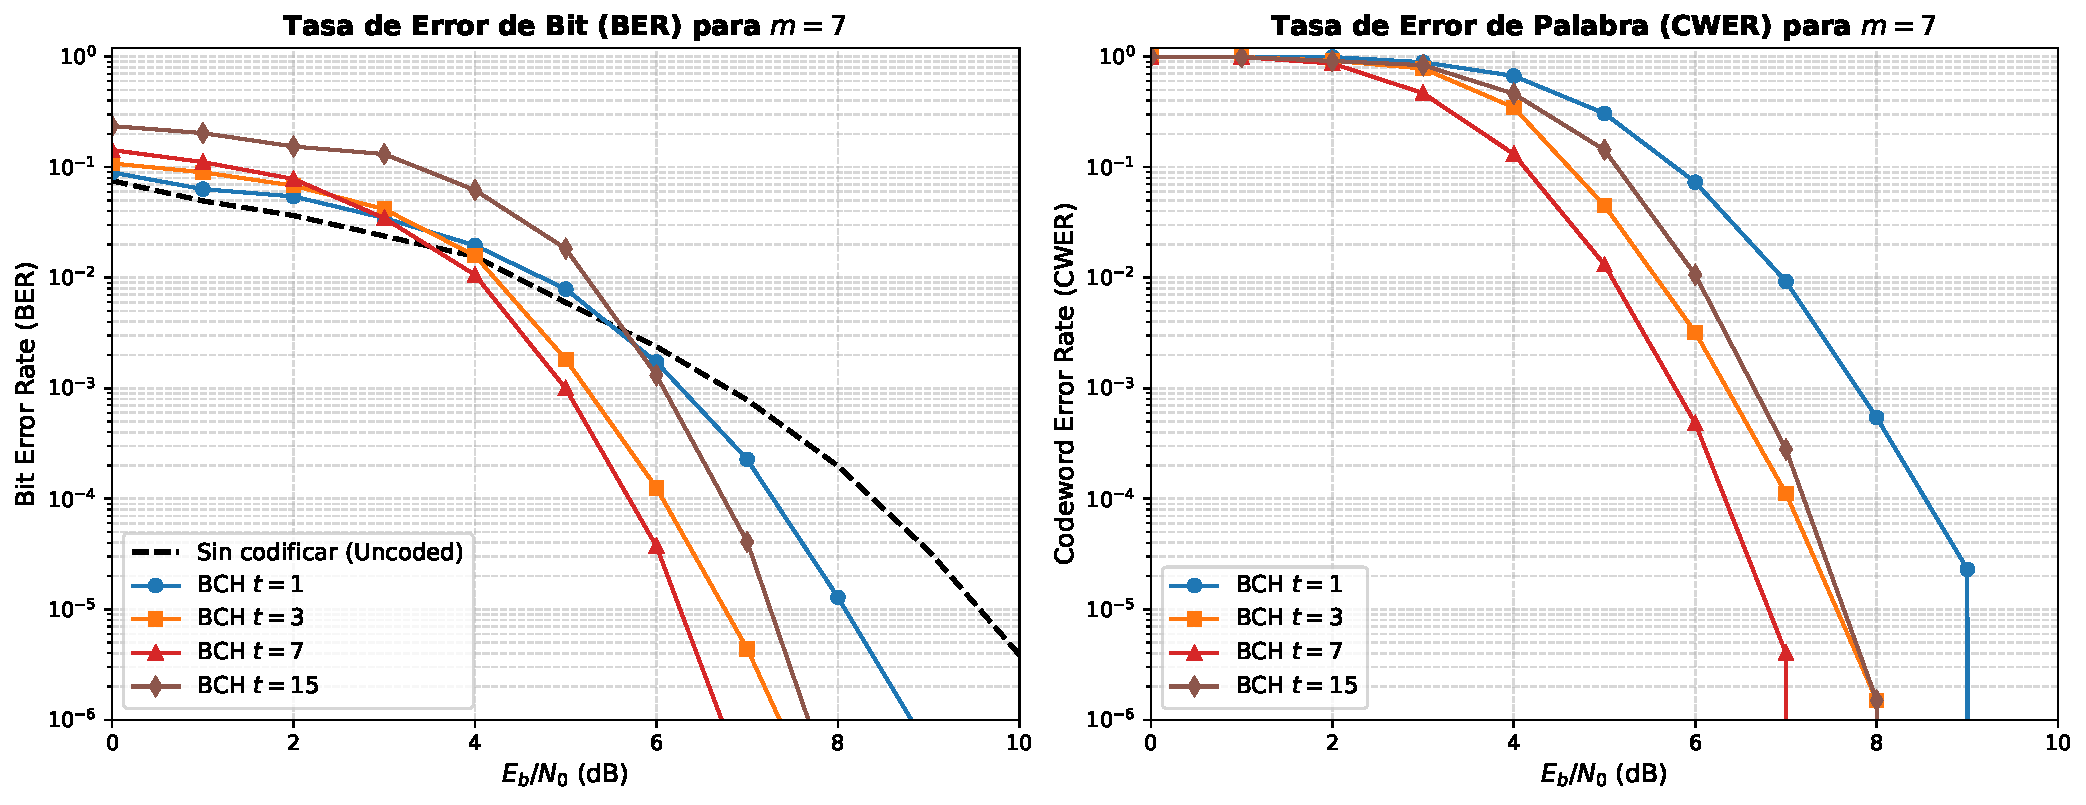
\includegraphics[width=1.0\textwidth]{../graficos/grafica_bch_m7.pdf}
    \caption{Estudio comparativo para $m=7$: Tasa de Error de Bit (BER, izquierda) y Tasa de Error de Palabra (CWER, derecha) para $t \in \{1, 3, 7, 15\}$.}
    \label{fig:rendimiento_m7}
\end{figure}

A partir de los resultados mostrados en la Figura \ref{fig:rendimiento_m7}, se pueden identificar tres comportamientos principales:

\subsection{Saturación del decodificador en entornos de alto ruido}

En condiciones de ruido elevado (aproximadamente entre 0 y 3 dB), se observa un comportamiento contraintuitivo: el código con mayor capacidad teórica de corrección ($t=15$) presenta la peor tasa de error de bit (BER). 

Esto ocurre porque su baja tasa de código ($R = 0,173$) obliga al canal a introducir un volumen mucho mayor de errores para mantener la misma energía por bit de información ($E_b/N_0$). Cuando el número de errores supera la capacidad de corrección, el algoritmo de Berlekamp-Massey genera un polinomio localizador incorrecto. El decodificador intenta entonces corregir posiciones erróneas, lo que añade más errores al bloque. Como consecuencia, la tasa de error de palabra (CWER) se acerca a 1 y la BER llega a ser incluso superior a la del canal sin codificar.

\subsection{Efecto umbral y coste de la redundancia}

A partir de unos 4 dB, las curvas muestran el típico «efecto umbral» de la decodificación algebraica con decisión dura. Sin embargo, un mayor valor de $t$ no siempre implica un mejor rendimiento.

La configuración $t=7$ ofrece el mejor comportamiento global: presenta la caída más rápida de la BER y desplaza el punto de convergencia hacia valores más bajos de $E_b/N_0$. Por el contrario, el código con $t=15$ mejora de forma más lenta y su curva está desplazada hacia la derecha respecto a $t=3$ y $t=7$.

Este resultado pone de manifiesto la \textbf{penalización por la tasa de código}. Aunque $t=15$ tiene mayor capacidad correctora, su elevada redundancia hace que el canal sea mucho más hostil, superando con frecuencia la capacidad real del decodificador.

\subsection{Diferencia entre BER y CWER}

La comparación de ambas gráficas muestra que la tasa de error de palabra (CWER) siempre desciende más lentamente que la tasa de error de bit (BER). Esto es lógico, ya que la CWER considera que un bloque completo ha fallado aunque solo quede un único bit erróneo, mientras que la BER mide el promedio de bits erróneos sobre el total de bits transmitidos.

\subsection{Conclusión}

Los resultados demuestran que el rendimiento del código no mejora de forma monótona al aumentar la capacidad de corrección $t$. Para $m=7$, existe un punto de equilibrio óptimo en torno a $t=7$, que ofrece una buena protección sin incurrir en la fuerte penalización que sufre $t=15$, ni quedarse corto como ocurre con $t=1$ y $t=3$.

Este análisis confirma que el diseño de un códec BCH eficaz requiere equilibrar adecuadamente la distancia de corrección con la tasa de código y la penalización energética asociada.

\section{Comparación de rendimiento entre códigos con tasa de código similar}

En esta sección se aborda la evaluación del rendimiento aislando el efecto de la penalización por tasa de código (\textit{code rate penalty}). Al comparar configuraciones con diferentes grados de extensión ($m$) pero que comparten una tasa de código ($R = k/n$) equivalente, la varianza del ruido en el canal físico ($\sigma^2$) se mantiene constante para cada valor de $E_b/N_0$ evaluado. Este diseño experimental permite analizar de forma directa el impacto de la longitud del bloque ($n$) y de la capacidad correctora ($t$) sobre la mitigación de errores.

A partir de los datos obtenidos, se han estructurado tres escenarios de evaluación (tasa alta, media y baja) basados en los grados de extensión $m \in \{5, 7, 11\}$, cuyos parámetros constructivos se detallan en la Tabla \ref{tab:tasas_similares}.

\begin{table}[h!]
\centering
\caption{Agrupación simétrica de códigos BCH bajo criterios de tasa de código similar.}
\label{tab:tasas_similares}
\resizebox{\textwidth}{!}{%
\begin{tabular}{cccccc}
\hline
\textbf{Escenario} & \textbf{Grado ($m$)} & \textbf{Bloque ($n$)} & \textbf{Capacidad ($t$)} & \textbf{Información ($k$)} & \textbf{Tasa ($R$)} \\ \hline
Tasa Alta          & 5                    & 31                    & 1                        & 26                         & 0,838               \\
($R \approx 0,82$) & 7                    & 127                   & 3                        & 106                        & 0,835               \\
                   & 11                   & 2047                  & 35                       & 1662                       & 0,812               \\ \hline
Tasa Media         & 5                    & 31                    & 3                        & 16                         & 0,516               \\
($R \approx 0,50$) & 7                    & 127                   & 9                        & 64                         & 0,504               \\
                   & 11                   & 2047                  & 93                       & 1024                       & 0,500               \\ \hline
Tasa Baja          & 5                    & 31                    & 5                        & 11                         & 0,355               \\
($R \approx 0,34$) & 7                    & 127                   & 14                       & 43                         & 0,338               \\
                   & 11                   & 2047                  & 124                      & 683                        & 0,334               \\ \hline
\end{tabular}%
}
\end{table}

\subsection{Análisis del rendimiento en función de la longitud de bloque}

El primer enfoque de este estudio se presenta en la Figura \ref{fig:tasas_similares_grafica}, donde las curvas de rendimiento se agrupan manteniendo una tasa de código similar en cada gráfica. De este modo, es posible observar la influencia intrínseca de la longitud del bloque sobre el comportamiento del sistema frente al ruido.

A partir de los resultados experimentales, se identifican dos tendencias fundamentales comunes a los tres escenarios evaluados:

\begin{itemize}

    \item \textbf{Efecto umbral y caída en cascada (\textit{waterfall}) en bloques largos:}  
    En todos los niveles de tasa de código, las configuraciones con bloques de mayor longitud ($m=11$) exhiben una pendiente de caída de la BER considerablemente más pronunciada. Aunque en regímenes de ruido intenso (valores bajos de $E_b/N_0$) su rendimiento es similar o ligeramente inferior al de los bloques cortos debido a la propagación de errores en ráfaga, una vez se supera un determinado umbral de relación señal-ruido, la BER disminuye drásticamente. Esto confirma que los códigos largos aprovechan con mayor eficiencia la redundancia conforme mejora el canal.

    \item \textbf{Robustez inicial y ganancia progresiva en bloques cortos:}  
    Por el contrario, las configuraciones cortas ($m=5$) muestran un comportamiento más lineal y estable en escenarios de baja relación señal-ruido, degradándose de forma menos abrupta. Sin embargo, al carecer de la pronunciada pendiente de caída característica de los códigos de gran longitud, estas configuraciones cortas requieren valores de $E_b/N_0$ notablemente más altos para alcanzar tasas de error muy bajas (por debajo de $10^{-4}$).

\end{itemize}

\begin{figure}[htbp]
    \centering
    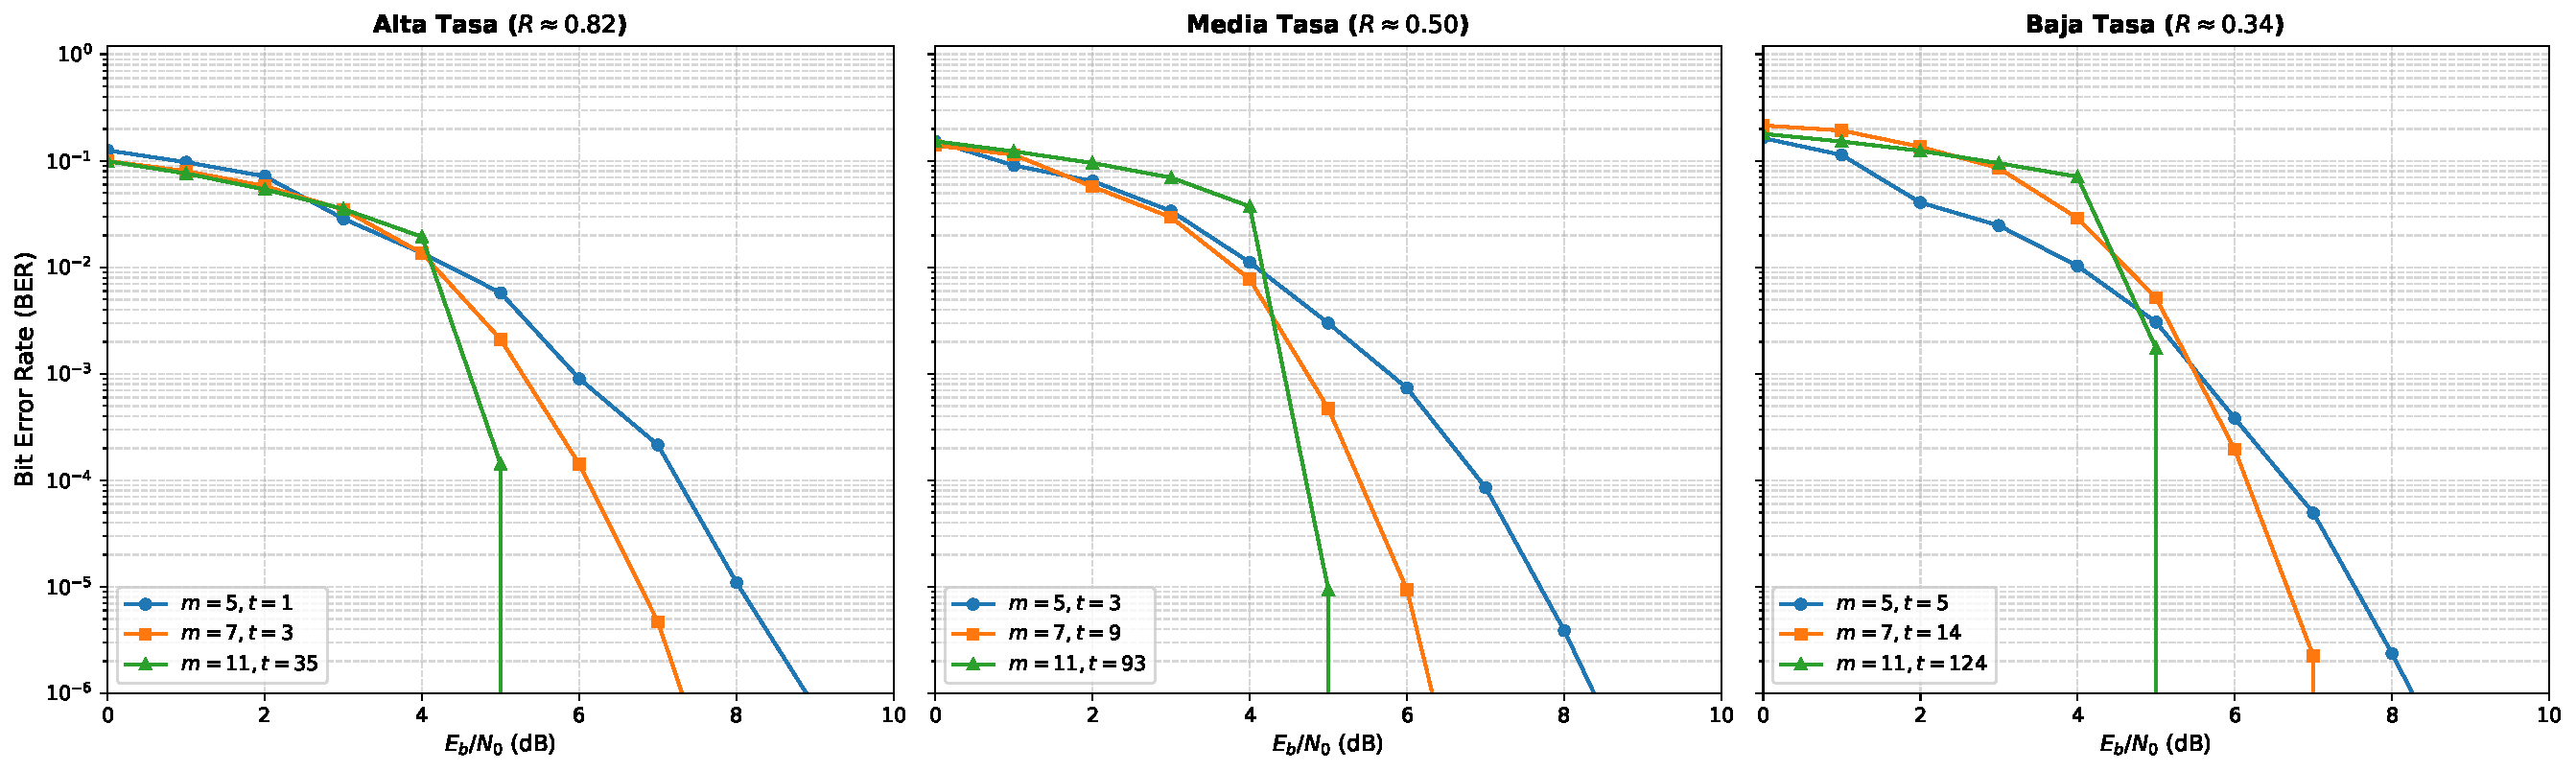
\includegraphics[width=1.0\textwidth]{../graficos/grafica_tasas_similares.pdf} 
    \caption{Estudio comparativo de la BER para agrupaciones de tasa similar: escenarios de tasa alta (izquierda), media (centro) y baja (derecha).}
    \label{fig:tasas_similares_grafica}
\end{figure}

\subsection{Análisis de sensibilidad según la capacidad correctora}

Para complementar el estudio previo, la Figura \ref{fig:correlacion_tasas} agrupa las curvas de rendimiento fijando el grado de extensión $m$ en cada subgráfica. Este enfoque permite aislar el impacto que produce el incremento de la capacidad correctora ($t$) —y la consecuente reducción de la tasa de código ($R$)— dentro de un mismo tamaño de bloque.

Los resultados experimentales demuestran que añadir redundancia no produce el mismo efecto en todos los horizontes de longitud de código:

\begin{itemize}

    \item \textbf{Bloques cortos ($m=5$):}  
    En este régimen, las tres configuraciones presentan un comportamiento prácticamente idéntico en la zona de relación señal-ruido baja y media (entre 0 y 6 dB), mostrando curvas que se solapan casi por completo. Esto evidencia que, para bloques tan cortos, incrementar la capacidad correctora de $t=1$ a $t=5$ apenas aporta una ganancia perceptible en la BER. Es a partir de los 6 dB donde la configuración de alta tasa ($t=1$, curva azul) comienza a degradarse y a distanciarse negativamente de las otras dos opciones. Por su parte, las curvas de tasa media ($t=3$) y baja ($t=5$) se mantienen pegadas en todo el recorrido; por tanto, la configuración intermedia ($t=3$) resulta la más eficiente a efectos prácticos, ya que logra el mismo límite de error que la opción con máxima redundancia pero sin penalizar la velocidad de transmisión de información útil.

    \item \textbf{Bloques intermedios ($m=7$):}  
    Aquí emerge un comportamiento no lineal respecto a la redundancia. La configuración de tasa media ($t=9$, curva naranja) ofrece el rendimiento óptimo del panel, exhibiendo la caída de BER más rápida. Por el contrario, saturar el bloque con mayor capacidad correctora ($t=14$, curva verde) resulta contraproducente: presenta el peor desempeño de la zona con ruido intenso (hasta los $6 \text{ dB}$) debido a la severa penalización de la tasa de código, y solo iguala a la configuración intermedia en el extremo de alta relación señal-ruido.

    \item \textbf{Bloques largos ($m=11$):}  
    Para códigos de gran longitud, el impacto de la penalización por tasa de código en entornos hostiles es muy evidente. En la zona de baja relación señal-ruido (de 0 a 4 dB), la configuración con máxima redundancia ($t=124$, curva verde) es superada de forma clara por las tasas media y alta, posicionándose como la opción con peor rendimiento. No obstante, en el intervalo entre los 4 y los 5 dB, esta tendencia cambia de manera drástica: la curva verde experimenta una caída en cascada vertical e instantánea. Al venir desde una zona de errores más elevada, protagoniza el descenso más significativo del panel, logrando que la BER caiga por debajo de $10^{-6}$ y converja en el límite de error cero en el mismo punto que las demás configuraciones en cuanto el canal empieza a despejarse.    
    
\end{itemize}

\begin{figure}[htbp]
    \centering
    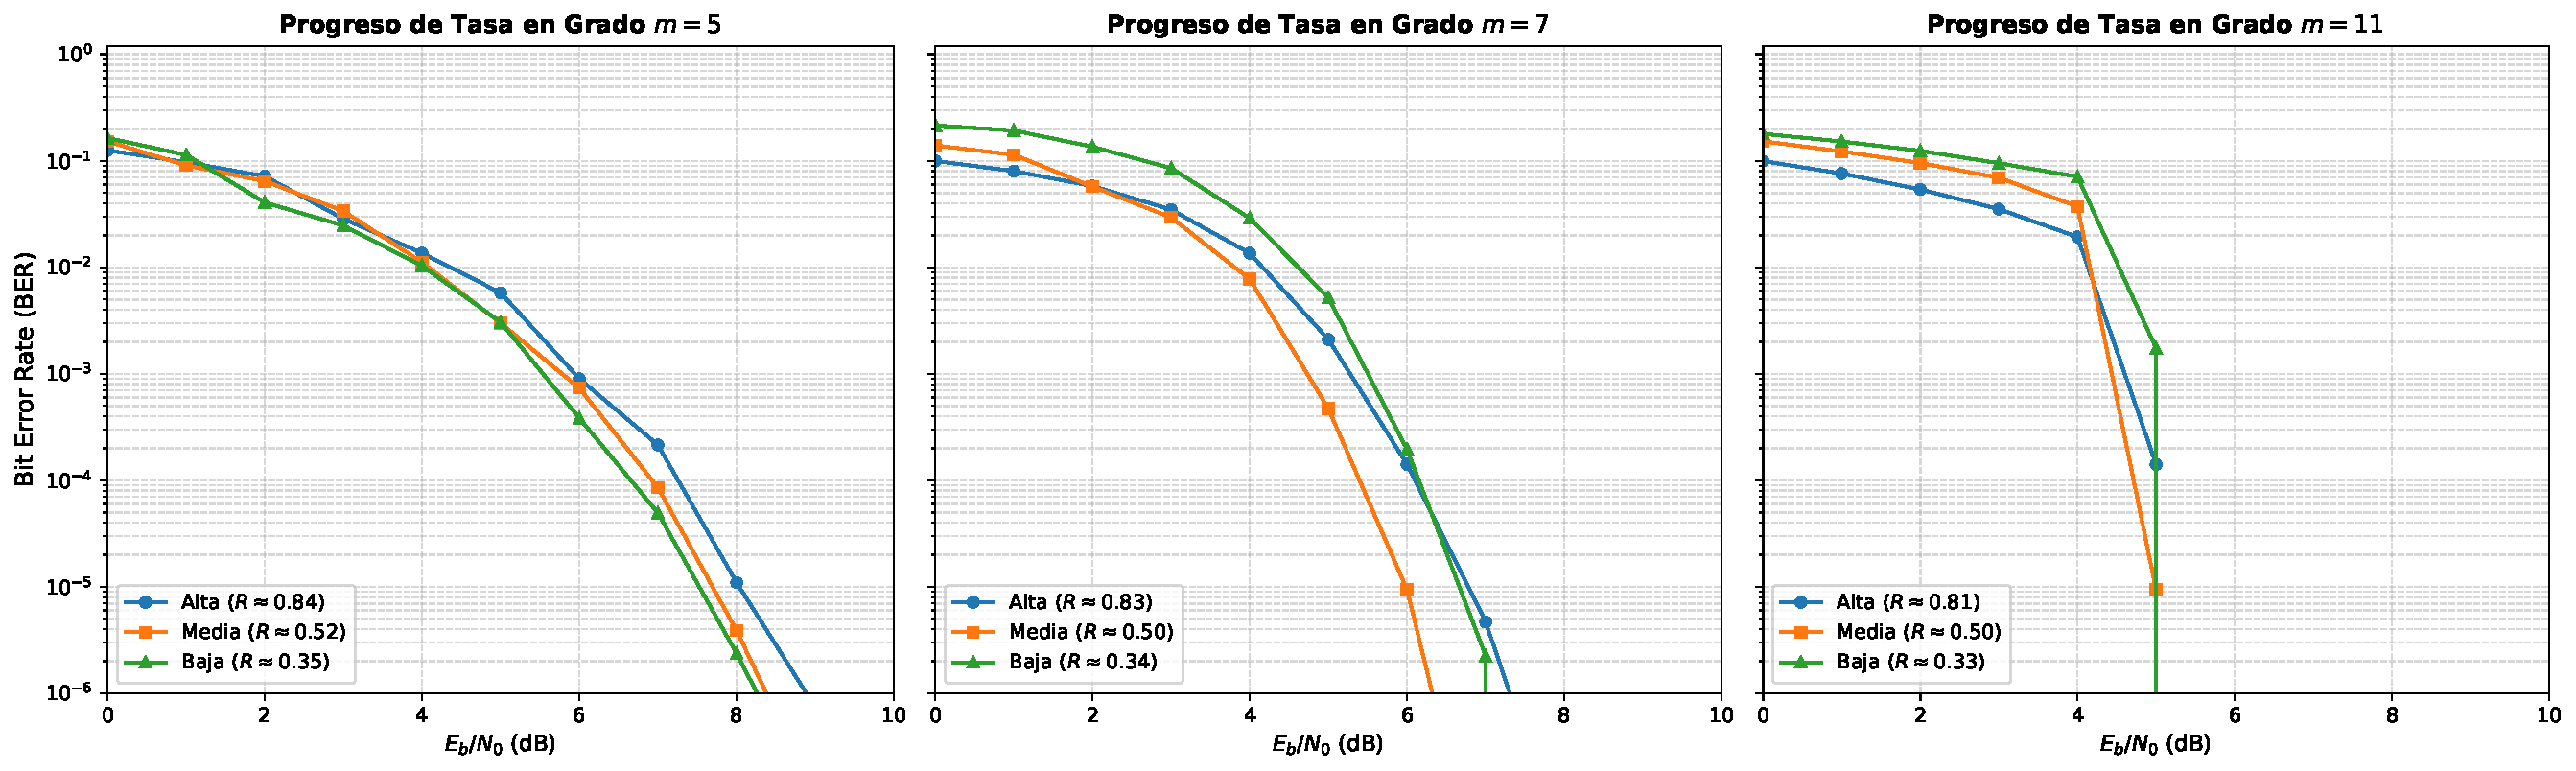
\includegraphics[width=1.0\textwidth]{../graficos/grafica_correlacion_tasas.pdf} 
    \caption{Estudio de sensibilidad de la tasa de código agrupado por grado de extensión: $m=5$ (izquierda), $m=7$ (centro) y $m=11$ (derecha).}
    \label{fig:correlacion_tasas}
\end{figure}


\subsection{Discusión global y criterios de diseño}

Los resultados obtenidos en los diferentes escenarios evidencian que el beneficio de incrementar la redundancia está condicionado por la longitud del bloque del código. En estructuras de bloques cortos ($m=5$), las curvas se solapan y añadir más paridad no aporta una ganancia apreciable frente al ruido. En cambio, en bloques intermedios ($m=7$) y largos ($m=11$), un exceso de bits de paridad penaliza severamente el rendimiento en canales degradados, requiriendo superar un umbral crítico de relación señal-ruido para activar su potencial de corrección en cascada.

En consecuencia, las simulaciones certifican la inexistencia de una solución universal y permiten definir criterios de diseño claros: si el sistema opera con restricciones de tamaño de bloque corto, la configuración de tasa media representa el compromiso óptimo, al igualar el rendimiento de la tasa baja sin penalizar la velocidad de transmisión. Por el contrario, si se implementan bloques largos en canales donde se garantiza superar los 5 dB, las configuraciones de alta tasa son las más eficientes, ya que logran la convergencia a error cero en el mismo umbral que las demás pero maximizando la tasa de transferencia de datos útiles.

\section{Evaluación del Rendimiento Computacional}
\label{sec:rendimiento_computacional}

La viabilidad práctica de un código corrector de errores no depende únicamente de su capacidad de corrección estadística, evaluada mediante métricas como BER y CWER, sino también de su coste computacional y de su latencia de procesamiento. Un sistema con excelentes prestaciones de corrección puede perder aplicabilidad práctica si el tiempo necesario para codificar o decodificar cada bloque resulta excesivo.

\subsection{Evolución de la latencia frente al estado del canal}
Con el objetivo de analizar este comportamiento, se ha evaluado una configuración BCH con parámetros $m=7$ y $t=10$, registrando el tiempo medio de procesamiento por palabra de código frente a distintos niveles de degradación del canal AWGN (Figura \ref{fig:latencia_m7_t10}).

\begin{figure}[htbp]
    \centering
    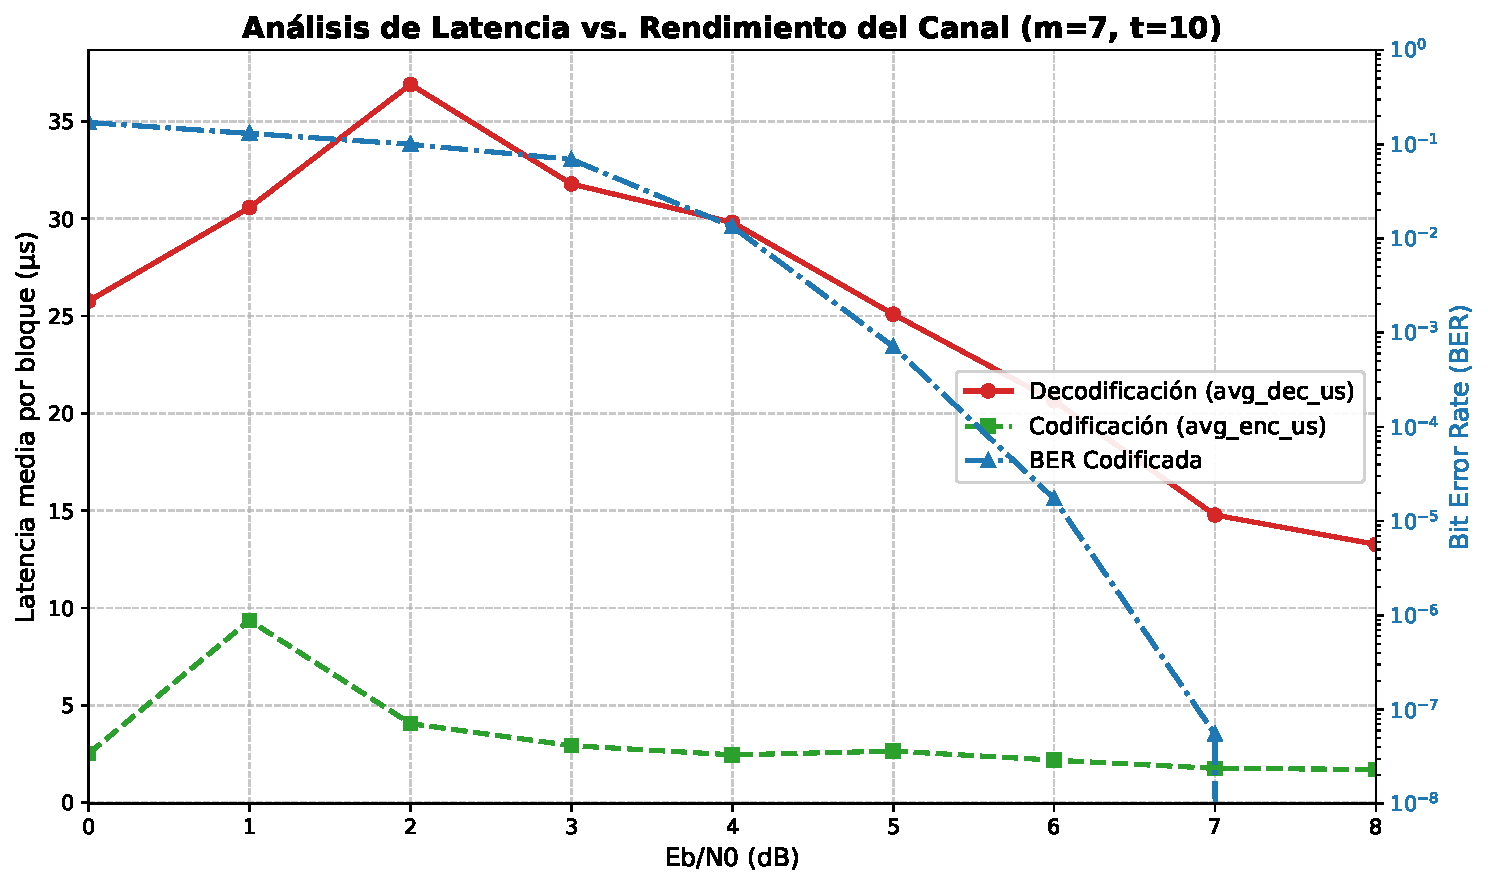
\includegraphics[width=1.0\textwidth]{../graficos/grafica_latencia_m7_t10.pdf}
    \caption{Coste computacional (eje izquierdo) frente al rendimiento del canal (eje derecho) para $m=7, t=10$.}
    \label{fig:latencia_m7_t10}
\end{figure}

Los resultados muestran un comportamiento claramente diferenciado entre los módulos de codificación y decodificación:

\begin{itemize}

    \item \textbf{Estabilidad en la codificación:}  
    La latencia de codificación (línea verde discontinua) permanece reducida y relativamente estable a lo largo de todo el rango de $E_b/N_0$, manteniéndose generalmente por debajo de los $5\,\mu s$. Aunque se observa un incremento puntual cercano a $1\,\text{dB}$, el comportamiento global confirma que el codificador apenas se ve afectado por las condiciones del canal, ya que siempre ejecuta la misma secuencia de operaciones. Además, el uso de la estructura \texttt{PackedBit} permite realizar operaciones XOR y desplazamientos sobre palabras de 64 bits, reduciendo significativamente el coste de la división polinómica binaria.
    \item \textbf{Dependencia de la decodificación respecto al canal:}  
    En contraste, la latencia de decodificación (línea roja continua) muestra una dependencia significativa del estado del canal. En condiciones de ruido elevado ($0\,\text{dB}$), el tiempo de ejecución ya resulta considerable debido a la elevada cantidad de errores presentes en cada bloque. Posteriormente, el sistema alcanza su máxima carga de trabajo en torno a $2\,\text{dB}$, donde la latencia supera los $35\,\mu s$. Esta región representa el escenario más exigente para el decodificador, ya que el algoritmo debe completar íntegramente las fases de cálculo de síndromes, Berlekamp--Massey y búsqueda de Chien antes de localizar las posiciones erróneas.

    \item \textbf{Disminución progresiva de la latencia:}  
    A medida que mejora la relación señal a ruido, la latencia de decodificación disminuye progresivamente hasta estabilizarse por debajo de los $15\,\mu s$ para valores elevados de $E_b/N_0$. Este comportamiento pone de manifiesto la eficacia del mecanismo de finalización anticipada implementado en el decodificador: cuando el vector de síndromes resulta nulo, el sistema evita ejecutar los posteriores algoritmos, reduciendo considerablemente el número de operaciones necesarias.

    \item \textbf{Relación entre BER y coste computacional:}  
    Además, la curva BER codificada presenta el comportamiento en cascada (\textit{waterfall effect}) característico de los códigos BCH. A partir de aproximadamente $4\,\text{dB}$, la tasa de error desciende varios órdenes de magnitud de forma abrupta, coincidiendo con la reducción observada en la latencia de decodificación. Esto indica que, bajo condiciones de canal favorables, el sistema no solo mejora su capacidad de corrección, sino también su eficiencia computacional.

\end{itemize}

\subsection{Impacto de la complejidad estructural del código}

Una vez analizado el impacto de las condiciones del canal sobre la latencia, se estudia ahora la influencia de la complejidad intrínseca del código BCH. En este caso, se mantiene fijo el canal AWGN y se varían los parámetros estructurales del código ($m$ y $t$), con el objetivo de evaluar su efecto sobre el coste computacional de los procesos de codificación y decodificación.

Los resultados, representados mediante el diagrama de barras agrupadas de la Figura \ref{fig:complejidad_m7}, muestran una clara asimetría entre los procesos de transmisión y recepción:

\begin{figure}[htbp]
    \centering
    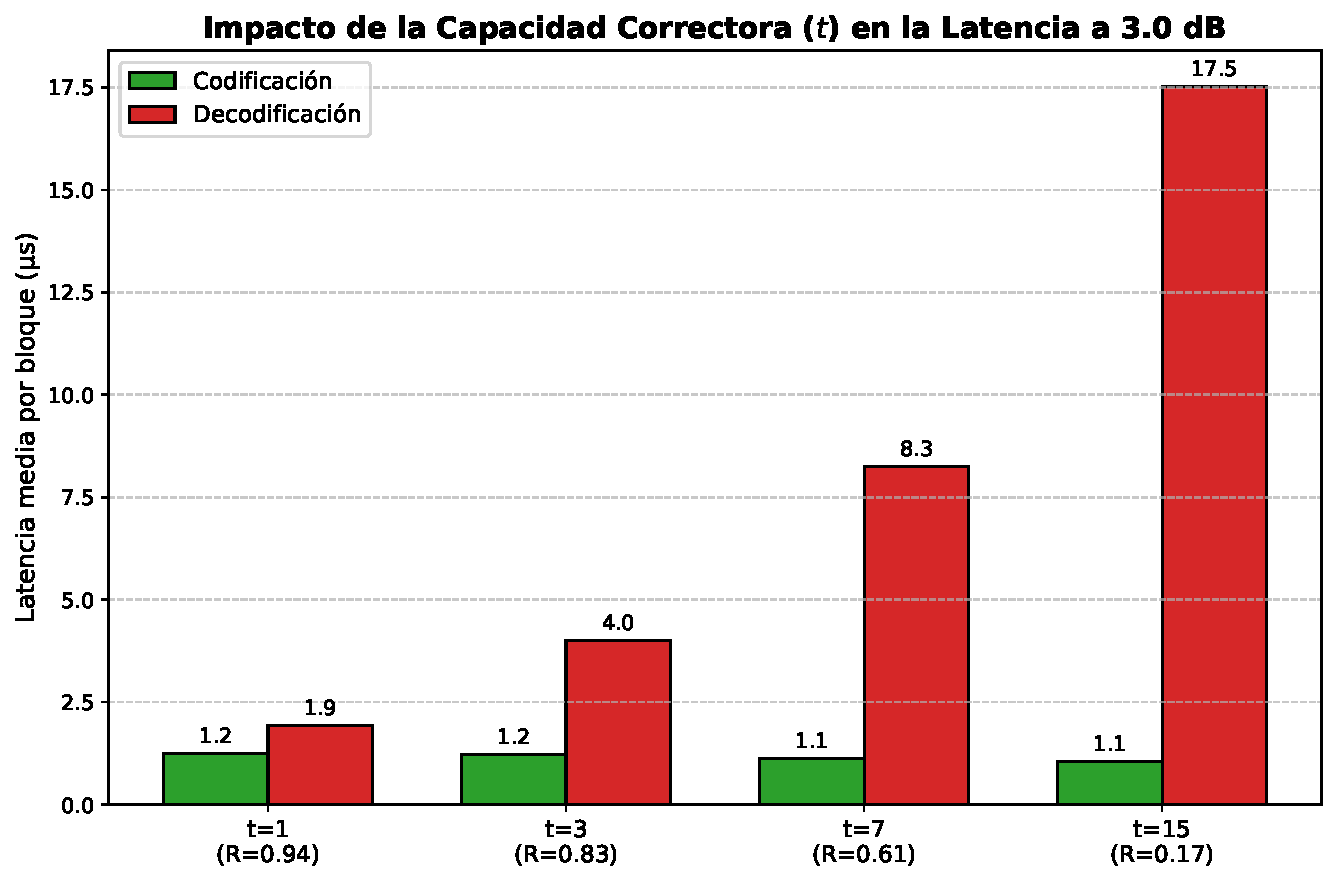
\includegraphics[width=1\textwidth]{../graficos/grafica_complejidad_m7.pdf}
    \caption{Comparativa de la latencia computacional en función de la capacidad correctora $t$ para $m=7$ a $3\,\text{dB}$.}
    \label{fig:complejidad_m7}
\end{figure}

\begin{itemize}

    \item \textbf{Codificación constante respecto a $t$:}  
    Como se observa en la gráfica, independientemente del número de bits de paridad introducidos (desde $R=0.94$ hasta $R=0.17$), el tiempo de codificación se mantiene prácticamente invariable, oscilando entre $1.1$ y $1.2\,\mu s$. Este comportamiento se explica porque la implementación basada en \texttt{PackedBit} realiza operaciones sobre palabras de 64 bits y el coste depende principalmente de la longitud del bloque $n$, que permanece constante en este estudio. Por tanto, la complejidad es independiente de $t$, aunque no estrictamente constante en términos absolutos.

    \item \textbf{Incremento de la latencia de decodificación con $t$:}  
    En contraste, la latencia de decodificación aumenta de forma significativa a medida que crece la capacidad correctora. Para $t=1$ la latencia es de aproximadamente $1.9\,\mu s$, mientras que para $t=15$ alcanza los $17.5\,\mu s$, lo que supone un incremento de casi un orden de magnitud. Este comportamiento es coherente con la complejidad de los algoritmos implicados:
    
    \begin{enumerate}
        \item El cálculo de síndromes depende del número de errores corregibles y escala proporcionalmente con $n$ y $2t$.
        \item El algoritmo de Berlekamp–Massey presenta una complejidad aproximada de $O(t^2)$ debido al crecimiento del polinomio localizador de errores.
        \item La búsqueda de raíces mediante el algoritmo de Chien requiere evaluar el polinomio localizador a lo largo de los $n$ elementos del cuerpo, lo que introduce una complejidad del orden de $O(n \cdot t)$.
    \end{enumerate}

\end{itemize}

En conclusión, los resultados muestran un compromiso de diseño claro: aumentar la capacidad correctora $t$ no solo reduce la tasa de código $R$, sino que incrementa de forma significativa el coste computacional del receptor. Este factor resulta especialmente relevante en aplicaciones donde la eficiencia energética o la latencia del sistema son restricciones críticas.

\section{Evaluación Cualitativa: Impacto Visual en la Transmisión de Imágenes}
\label{sec:impacto_visual}

Además del análisis estadístico basado en las curvas de rendimiento, resulta de gran utilidad evaluar cualitativamente el impacto del ruido en un escenario práctico de transmisión de datos. Para ello, se ha procesado una imagen en formato de mapa de bits (\texttt{.bmp}) utilizando la configuración $m=7$ y $t=7$. El uso de este formato, que carece de compresión espacial, permite observar de forma directa la degradación a nivel de píxel sin los artefactos que introducen algoritmos como JPEG.

\subsection{Evolución de la corrección frente al ruido}

En esta prueba se comparan las imágenes recibidas a través del canal sin codificar frente a las procesadas por el decodificador BCH para tres valores distintos de relación señal a ruido ($E_b/N_0$), lo que permite observar la evolución en la capacidad de recuperación del sistema.

\begin{figure}[htbp]
    \centering
    % Fila 1: 4 dB
    \begin{minipage}{0.48\textwidth}
        \centering
        
\includegraphics[width=\linewidth]{../imagenes/uncoded_EbNo_4_logo_ugr.png}
        \vspace{0.15cm}
        
        {\small a) Sin codificar (4 dB)}
    \end{minipage}\hfill
    \begin{minipage}{0.48\textwidth}
        \centering
        
\includegraphics[width=\linewidth]{../imagenes/out_EbNo_4_logo_ugr.png}
        \vspace{0.15cm}
        
        {\small b) BCH $t=7$ (4 dB)}
    \end{minipage}

    \vspace{0.4cm} % Espacio entre filas

    % Fila 2: 5 dB
    \begin{minipage}{0.48\textwidth}
        \centering
        
\includegraphics[width=\linewidth]{../imagenes/uncoded_EbNo_5_logo_ugr.png}
        \vspace{0.15cm}
        
        {\small c) Sin codificar (5 dB)}
    \end{minipage}\hfill
    \begin{minipage}{0.48\textwidth}
        \centering
        
\includegraphics[width=\linewidth]{../imagenes/out_EbNo_5_logo_ugr.png}
        \vspace{0.15cm}
        
        {\small d) BCH $t=7$ (5 dB)}
    \end{minipage}

    \vspace{0.4cm} % Espacio entre filas

    % Fila 3: 6 dB
    \begin{minipage}{0.48\textwidth}
        \centering
        
\includegraphics[width=\linewidth]{../imagenes/uncoded_EbNo_6_logo_ugr.png}
        \vspace{0.15cm}
        
        {\small e) Sin codificar (6 dB)}
    \end{minipage}\hfill
    \begin{minipage}{0.48\textwidth}
        \centering
        
\includegraphics[width=\linewidth]{../imagenes/out_EbNo_6_logo_ugr.png}
        \vspace{0.15cm}
        
        {\small f) BCH $t=7$ (6 dB)}
    \end{minipage}

    \caption{Comparativa visual de la transmisión de la imagen a 4 dB, 5 dB y 6 dB. Columna izquierda: canal sin codificar. Columna derecha: corrección mediante BCH.}
    \label{fig:prueba_fases_bch}
\end{figure}
\subsubsection{Comportamiento a 4 dB: Corrupción de cabeceras}
En condiciones de ruido elevado, la transmisión de datos estructurados presenta el problema de la corrupción de metadatos. Como se muestra en la Figura \ref{fig:prueba_fases_bch}a, la imagen sin codificar a $4\text{ dB}$ resulta ilegible para el sistema operativo. Este error se produce porque el ruido altera los bytes correspondientes a la cabecera del formato BMP, lo que impide la correcta lectura del archivo. Por el contrario, el código BCH logra proteger esta información estructural (Figura \ref{fig:prueba_fases_bch}b), permitiendo abrir el archivo y recuperar la imagen. No obstante, la imagen resultante aún presenta ruido visible, dado que la cantidad de errores introducidos por el canal supera en algunas palabras la capacidad correctora de $t=7$.

\subsubsection{Comportamiento a 5 dB: Reducción del error visual}
Al incrementar la relación señal a ruido a $5\text{ dB}$, la probabilidad de error del canal disminuye. En el caso sin codificar (Figura \ref{fig:prueba_fases_bch}c), la cabecera del archivo no resulta dañada, lo que permite visualizar la imagen y confirmar la presencia de alteraciones aleatorias en los píxeles. Por su parte, la imagen procesada por el decodificador BCH (Figura \ref{fig:prueba_fases_bch}d) evidencia una corrección mayoritaria de la información, eliminando la mayor parte del ruido y dejando únicamente algunos píxeles erróneos residuales.

\subsubsection{Comportamiento a 6 dB: Recuperación completa}
Para un nivel de $6\text{ dB}$, la transmisión sin codificar (Figura \ref{fig:prueba_fases_bch}e) sigue presentando errores que reduden la calidad final de la imagen. Sin embargo, la decodificación BCH (Figura \ref{fig:prueba_fases_bch}f) es capaz de corregir todos los errores introducidos en la señal. El resultado es una reconstrucción idéntica a la imagen original, alcanzando un estado de cero errores tras el proceso de decodificación.

\subsection{El coste de la redundancia: Degradación por exceso de paridad}

Uno de los fenómenos más notables observados en el análisis estadístico es que, en condiciones de ruido intenso, incrementar la capacidad teórica de corrección ($t$) puede resultar perjudicial. Para ilustrar visualmente este efecto, conocido como penalización por tasa de código (\textit{code rate penalty}), se ha simulado la transmisión de la imagen a un nivel de $E_b/N_0 = 5\text{ dB}$, comparando el canal sin codificar, una configuración equilibrada ($m=7, t=7$) y una de altísima redundancia ($m=7, t=15$).

La Figura \ref{fig:prueba_redundancia} presenta los resultados de esta comparativa.

\begin{figure}[htbp]
    \centering
    
    % Imagen Original
    
\includegraphics[width=0.85\textwidth]{../imagenes/logo_ugr.jpg}
    \vspace{0.15cm}
    
    {\small a) Imagen Original}
    
    \vspace{0.4cm} % Espacio entre imágenes
    
    % Sin codificar
    
\includegraphics[width=0.85\textwidth]{../imagenes/uncoded_EbNo_5_logo_ugr.png} 
    \vspace{0.15cm}
    
    {\small b) Sin codificar (5 dB)}
    
    \vspace{0.4cm}
    
    % BCH t=7
    
\includegraphics[width=0.85\textwidth]{../imagenes/out_EbNo_5_m7_t7_logo_ugr.png} 
    \vspace{0.15cm}
    
    {\small c) BCH $t=7$ (5 dB)}
    
    \vspace{0.4cm}
    
    % BCH t=15
    
\includegraphics[width=0.85\textwidth]{../imagenes/out_EbNo_5_m7_t15_logo_ugr.png} 
    \vspace{0.15cm}
    
    {\small d) BCH $t=15$ (5 dB)}

    \caption{Impacto visual de la penalización por tasa de código a $5\text{ dB}$. Al apilar las imágenes se aprecia claramente cómo la saturación de bits de paridad en $t=15$ genera una imagen más degradada que la propia transmisión sin codificar.}
    \label{fig:prueba_redundancia}
\end{figure}

Como se observa al comparar la transmisión sin codificar (Figura \ref{fig:prueba_redundancia}b) con el código BCH de $t=7$ (Figura \ref{fig:prueba_redundancia}c), la configuración equilibrada logra proteger la estructura del archivo y corregir la inmensa mayoría de la señal. La degradación visual es mínima, limitándose a errores residuales muy finos que se manifiestan como puntos de color aislados. 

Sin embargo, el comportamiento verdaderamente interesante se revela en la Figura \ref{fig:prueba_redundancia}d, correspondiente a la configuración $t=15$. A pesar de utilizar el código con la mayor capacidad correctora teórica, el resultado es severamente inferior, cubriendo la imagen con un denso ruido. De hecho, la imagen resultante presenta una calidad visual notablemente peor que la obtenida sin aplicar ninguna codificación.

Esta degradación es consecuencia directa de la baja tasa de código para $t=15$ ($R=0,173$). Para mantener la relación $E_b/N_0$ en $5\text{ dB}$, el simulador físico debe aumentar significativamente la varianza del ruido ($\sigma^2$). Este exceso de ruido de canal provoca que el número de errores físicos por bloque exceda de forma recurrente el límite de 15 bits, haciendo que el algoritmo de Berlekamp-Massey converja hacia polinomios localizadores erróneos. El decodificador procede entonces a invertir bits en posiciones equivocadas, alterando los canales de color del mapa de bits e introduciendo activamente más ruido del que el propio canal habría generado por sí solo.

\subsection{Impacto espacial: Distribución del error según la longitud del bloque}

Como última prueba de evaluación cualitativa, se analiza cómo la geometría matemática del código altera la estructura visual del error en el receptor. En el análisis estadístico de tasas similares, se demostró que los códigos largos presentan caídas abruptas de BER, mientras que los cortos tienen una degradación más suave. Para visualizar este fenómeno, se ha transmitido la imagen a un nivel de $4\text{ dB}$ utilizando dos configuraciones de Tasa Media ($R \approx 0.50$): bloques cortos ($m=5, t=3$) y bloques largos ($m=11, t=93$).

La Figura \ref{fig:prueba_topologia} presenta los resultados de esta comparativa.

\begin{figure}[htbp]
    \centering
    
    % Bloques Cortos (m=5)
    
\includegraphics[width=0.85\textwidth]{../imagenes/out_EbNo_4_m5_t3.png} 
    \vspace{0.15cm}
    
    {\small a) Bloques cortos: BCH $m=5, t=3$ ($n=31$ bits)}
    
    \vspace{0.6cm} % Espacio generoso entre imágenes
    
    % Bloques Largos (m=11)
    
\includegraphics[width=0.85\textwidth]{../imagenes/out_EbNo_4_m11_t93.png} 
    \vspace{0.15cm}
    
    {\small b) Bloques largos: BCH $m=11, t=93$ ($n=2047$ bits)}

    \caption{Distribución espacial del error a $4\text{ dB}$. Arriba: Ruido fino y disperso debido al fallo de bloques pequeños. Abajo: Errores en ráfaga (rayas horizontales) por el colapso de bloques grandes.}
    \label{fig:prueba_topologia}
\end{figure}

Como se observa en la Figura \ref{fig:prueba_topologia}a, la configuración de bloques cortos ($m=5$) genera una distribución de errores fina y dispersa, asimilable a un ruido impulsivo tradicional. Esto se debe a que la longitud de palabra es de apenas $31\text{ bits}$. Cuando el ruido del canal supera la capacidad correctora de $t=3$ y el decodificador falla, la corrupción se limita a unos pocos píxeles adyacentes, distribuyendo el daño de forma homogénea por toda la imagen.

En marcado contraste, la Figura \ref{fig:prueba_topologia}b muestra el resultado para la configuración de bloques largos ($m=11$). Su longitud de palabra es masiva ($2047\text{ bits}$, abarcando decenas de píxeles consecutivos). A $4\text{ dB}$, el sistema se encuentra justo en el límite de su efecto cascada. Cuando un bloque sobrevive, decodifica un segmento de la imagen con absoluta limpieza. Sin embargo, cuando el ruido supera el umbral de $t=93$, el fallo del algoritmo de Berlekamp-Massey corrompe el bloque completo. El resultado visual es la propagación de errores en ráfaga, manifestándose como evidentes rayas o franjas horizontales de ruido intenso intercaladas con franjas de imagen perfecta.

Esta evaluación demuestra que la longitud del bloque ($n$) no solo altera las métricas estadísticas, sino que define cómo se manifiestan realmente los errores en los datos. Este es un factor fundamental que debe tenerse en cuenta dependiendo del tipo de información que se vaya a transmitir.